\section{Leerlaufversuch}
Der Leerlaufversuch dient der Bestimmung der Leerlaufverluste,  welche sich aus den Eisenverlusten (Hystere- und Wirbelstromverlusten) sowie Zusatzverlusten (Streuflüssen bei  unsymmetrischen Bauformen) ergeben. Die Kupferverluste können bei dieser Messung aufgrund des geringen Leerlaufstromes vernachlässigt werden. Für die Durchführung ist nur die Primärseite des Transformators verschaltet, während die Sekundärseite offen bleibt. Die entsprechende allpolige Messchaltung ist in Abbildung\;\ref{fig:Leerlauf_3straengig} ersichtlich, das einsträngige Ersatzschaltbild in Abbildung\;\ref{fig:Leerlauf_ESB_1straengig}.\\
\begin{figure}[h!]
    \centering
    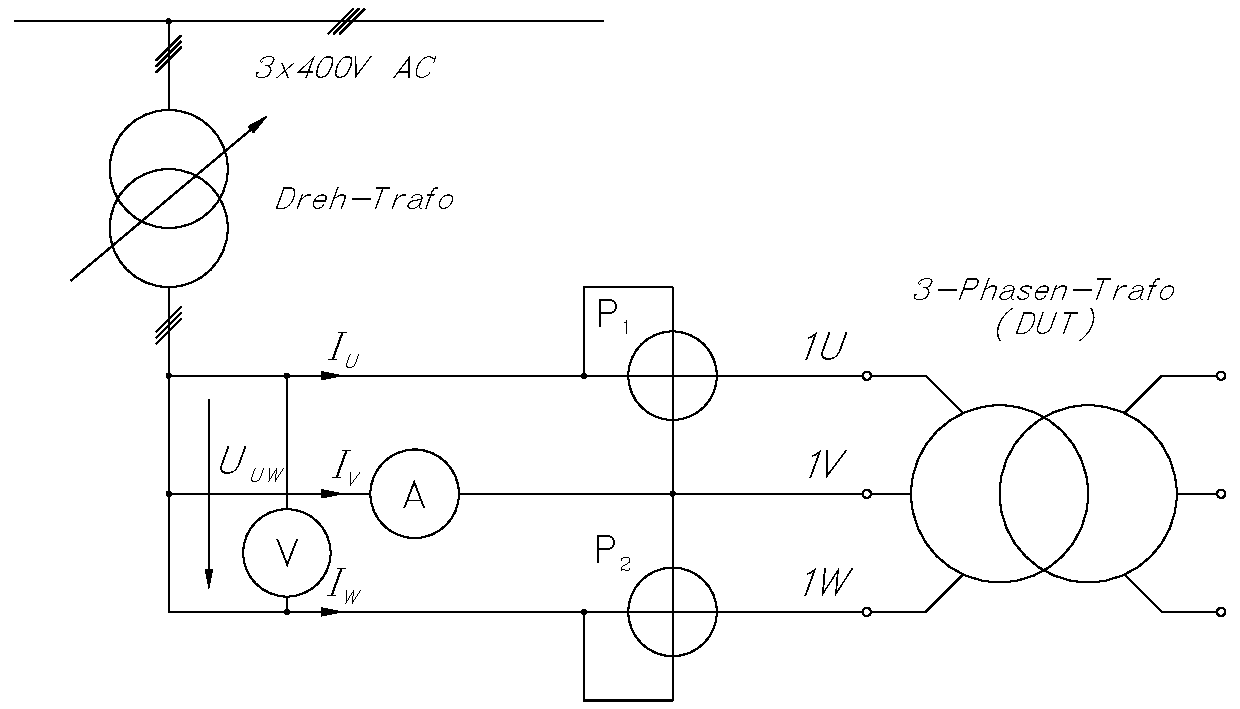
\includegraphics[width=0.75\textwidth, angle=0]{1/images/Leerlauf_3straengig.pdf}
    \caption{Messchaltung für den Leerlaufversuch; Messung der von der Oberspannungswicklung aufgenommenen Wirkleistung mit der 2-Watt-Meter-Methode (bzw. zusätzlicher Strom- und Spannungsmessung) bei offener Unterspannungswicklung.}
    \label{fig:Leerlauf_3straengig}
\end{figure}
\begin{figure}[h!]
    \centering
    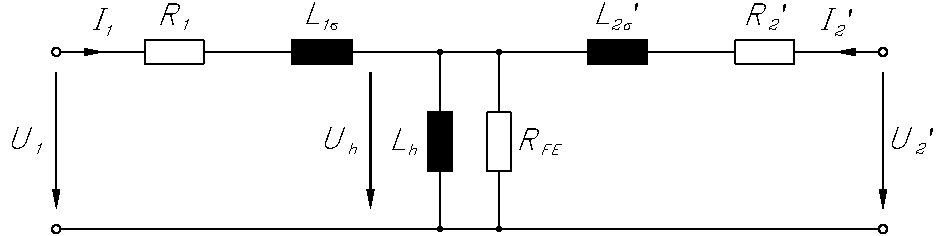
\includegraphics[width=0.75\textwidth, angle=0]{1/images/ESB_1straengig.pdf}
    \caption{1-Strängiges Ersatzschaltbild eines Transformators mit Kupferwiderständen ($R_1, R_2'$) und Streureaktanzen ($L_{1\sigma}, L_{2\sigma}'$) der Ober- und Unterspannungswicklung bzw. Hauptinduktivität $L_h$ und Eisenverlustwiderstand $R_{FE}$.}
    \label{fig:Leerlauf_ESB_1straengig}
\end{figure}
\noindent 
Bei der Messung werden alle Außenleiterspannungen $U_{AL,0}$ und Strangströme $I_{Str,0}$ (=Außenleiterströme $I_{AL,0}$ aufgrund primärer Sternschaltung) sowie die Wirkleistung $P_0$ der Primärseite gemessen und für die Berechnungen die jeweils gemittelten Werte genutzt. 
Die primäre Außenleiterspannung wird vom 1,2-fachen des Nennwertes ausgehend verringert. Aus den gemessenen Werten werden die Scheinleistung $S_0$ und der Leistungsfaktor $\cos{(\phi_0)}$ berechnet. Eine Übersicht über sämtliche Werte liefert Tabelle \ref{tab:leerlauf_werte}. 

\begin{table}[htb]
     \begin{center}
\begin{tabular}{|c|c|c|c|c|c|}
     \hline
     $U_{AL,0,avg} [\si{V}]$ & $I_{0,avg} [\si{A}]$ & $i_{m} [1]$ & $P_0 [\si{W}]$ & $S_0 [\si{VA}]$ & $\cos{(\phi_0)} [1]$ \\
     \hline \hline
     450.33 & 22.87 & 0.301 & 1500.00 & 17836.00 & 0.08\\ \hline
     401.00 & 12.75 & 0.168 & 1200.00 & 8855.54 & 0.14\\ \hline
     380.67 & 10.01 & 0.132 & 900.00 & 6597.74 & 0.14\\ \hline
     350.67 & 6.98 & 0.092 & 660.00 & 4237.44 & 0.16\\ \hline
     302.00 & 3.57 & 0.047 & 430.00 & 1869.14 & 0.23\\ \hline
     250.67 & 1.54 & 0.020 & 270.00 & 667.17 & 0.40\\ \hline
     200.67 & 0.85 & 0.011 & 168.00 & 294.27 & 0.57\\ \hline
     150.67 & 0.56 & 0.007 & 97.00 & 145.27 & 0.67\\ \hline
     100.60 & 0.39 & 0.005 & 44.00 & 68.54 & 0.64\\ \hline
     50.20 & 0.25 & 0.003 & 11.00 & 22.03 & 0.50\\ \hline
     10.03 & 0.14 & 0.002 & 0.00 & 2.49 & 0.00\\
     \hline
\end{tabular}
\end{center}
\label{tab:leerlauf_werte}
\caption{Gemessene und berechnete Werte für den Leerlaufversuch (avg=average, gemittelter Wert).}
\end{table}

\noindent In Abbildung \ref{fig:leerlauf_leistungen} sind die Wirk- und Scheinleistung sowie der Leistungsfaktor, in Abbildung \ref{fig:leerlauf_spannung} die gemittelte Leerlaufspannung in Abhängigkeit des gemittelten Leerlaufstromes ersichtlich.

\input{\currfiledir leerlauf}
\input{\currfiledir leerlauf_spannung}

\noindent
Es ist deutlich die erwartete Sättigung des Trafoblechs zu erkennen. Die Flussverkettung wird aufgrund des Induktionsgesetzes durch die Außenleiterspannung vorgegeben, und um diese zu erreichen, bedarf es ab dem nichtlinearen, gesättigten Bereich laut dem Durchflutungssatz eines überproportionalen Magnetisierungsstroms. Damit einher geht ein stark erhöhter Blindleistungsbedarf, der den Leistungsfaktor mit steigender Leerlaufspannung bzw. zunehmendem Magnetisierungsstrom stark sinken lässt. Dies ist auch durch das einsträngige Ersatzschaltbild ersichtlich, wenn man bedenkt, dass durch die Sättigung des Trafoblechs die Hauptfeldreaktanz geringer wird und in der Parallelschaltung folglich mehr Strom über den induktiven Zweig fließt.  
\noindent Abbildung \ref{fig:leerlauf_stroeme} zeigt den Zeitverlauf der Strangströme in einem sättigenden Arbeitspunkt. Die deutlich erkennbare Verzerrung im Vergleich zu einem sinusförmigen Verlauf rührt aus Oberschwingungen, die ihren Ursprung in der nichtlinearen Charakteristik der Magnetisierungskennlinie haben. Weiters ist erkennbar, dass der Magnetisierungsstrom des geometrisch mittleren Schenkels betraglich geringer ist als jene der äußeren Schenkel, was aus einem geometrisch bedingten geringeren Magnetisierungsbedarf resultiert.  
Im Leerlauf kann der Längszweig des Ersatzschaltbildes (Abb.\;\ref{fig:Leerlauf_ESB_1straengig}) vernachlässigt werden, womit aus den Messergebnissen des Leerlaufversuches der Magnetisierungsstrom und die Eisenverluste abgeschätzt werden können.
\begin{equation}
    I_\mu = \frac{Q_0}{3\cdot U_{N,S}}=\frac{\sqrt{S_0^2-P_0^2}}{\sqrt{3}\cdot U_{AL,0,avg}}=\frac{6536\,VA}{\sqrt{3}\cdot \SI{380}{\volt}}=\SI{9.93}{\ampere}
\end{equation}
\begin{equation}
    i_\mu = \frac{I\mu}{I_{N,S}}=\frac{\SI{9.93}{\ampere}}{\SI{76}{\ampere}}=0,131=13,1\%.
\end{equation}
Die Nenneisenverluste entsprechen (nach Vernachlässigung der Kupferverluste) der vom Transformator bei Bemessungsspannung aufgenommenen Wirkleistung
\begin{equation}
    P_{N,FE}=\SI{900}{\watt},
\end{equation}
woraus der Eisenverlustwiderstand abgeschätzt werden kann:
\begin{equation}
    R_{FE}=\frac{3\cdot U_{N,S}^2}{P_{FE}}=\frac{U_{AL,0,avg}^2}{P_{FE}}=\SI{160}{\ohm}.
\end{equation}
\input{\currfiledir zeitverlauf}